\documentclass[../the.tex]{subfiles}


\begin{document}


\section{Đặt vấn đề}
\label{tong_quan}

{\fontsize{13}{12} \selectfont

Ô nhiễm rác là tình trạng ô nhiễm phát sinh khi rác thải không được xử lí đúng cách hay rác thải được thu gom từ các bãi phế liệu bị bốc mùi hôi. Từ đó, chúng gây ảnh hưởng và làm ô nhiễm không khí ở các khu vực xung quanh. Ngoài ra tình trạng này cũng thể hiện khi rác thải được đốt cháy khiến các khí thải độc hại, khói bay ra gây ô nhiễm không khí và ảnh hưởng xấu tới sức khỏe con người, hệ động, thực vật.

}

\bigskip

{\fontsize{13}{12} \selectfont

Ô nhiễm môi trường bằng rác thải vẫn đang là vấn đề gây nhức nhối ở toàn cầu. Theo thống kê ở những nước có tốc độ đô thị hóa nhanh và dân số đông thì lượng rác thải sản sinh ra ngày càng nhiều. Ngày nay, Trung Quốc và Ấn Độ là những nước đứng đầu về việc ô nhiễm môi trường từ rác thải\footnote[1]{https://worldpopulationreview.com/country-rankings/plastic-pollution-by-country}.

}

\bigskip

{\fontsize{13}{12} \selectfont

Ở Việt Nam, hằng năm thải ra hơn 28 triệu tấn rác thải, tương đương 0,3kg bình quân mỗi người một ngày, với 76\% trong đó được ném ra các bãi rác tập trung. Sự thiếu phân loại từng loại rác, cùng với vấn đề của chất hữu cơ và độ ẩm cao khiến cho việc tái chế chất thải hỗn hợp thành nguyên liệu thô hoặc thành năng lượng trở nên khó khăn, điều này phần nào giải thích được tại sao các bãi rác thải tập trung có lượng rác chưa được xử lí với tỉ lệ cao\footnote[2]{https://woimacorporation.com/ngap-trong-rac-thai-van-de-dang-dien-ra-o-viet-nam}. Ở đô thị, mọi người dễ dàng bắt gặp được tình trạng các túi rác, ni lông, chai nhựa nằm rải rác trên các vỉa hè hay thậm chí dưới lòng đường. Điều đó gây mất cảnh quan đô thị, ảnh hưởng xấu đến chất lượng đời sống. Việt Nam đã phát triển một kế hoạch tập trung vào vấn đề tái chế và xử lí chất thải vào năm 2025 với hi vọng sẽ thu gom và xử lí tới 90\% chất thải rắn tại các thành phố, cùng với đó là tái chế hoặc tái sử dụng 85\% của chất thải rắn đế sản xuất năng lượng hoặc phân bón hữu cơ\footnote[3]{https://woimacorporation.com/ngap-trong-rac-thai-van-de-dang-dien-ra-o-viet-nam}. Việc chính quyền địa phương nắm được tình trạng phân loại, xả rác ở từng vùng, con phố sẽ giúp rất nhiều vào việc tái chế. Với sự phát triển của công nghệ thông tin nói chung và máy học nói riêng, việc áp dụng kỹ thuật học sâu vào phân loại rác thải dựa trên những hình ảnh trên đường phố sẽ giúp rút ngắn thời gian phát hiện và phân loại rác. Từ đó đưa ra được số liệu thống kê tình trạng phân bố của từng loại rác thải ở từng địa phương.

}

\bigskip

{\fontsize{13}{12} \selectfont 

Hiện nay, với sự phát triển của học sâu và ngân hàng các bộ dữ liệu về rác cũng rất phổ biến, có nhiều nghiên cứu cho thấy hiệu quả trong vấn đề phân lớp \cite{yang2016classification} \cite{shah2022method} \cite{ahmad2020intelligent}. 
Tuy nhiên vấn đề đặt ra là việc rác thải ở tự nhiên có thể bị biến dạng, phân mảnh hoặc bị chồng chéo lên nhau.
Các kết cấu tự nhiên như cát, đá, cỏ cây, vật thể trộn lẫn với rác làm cho các nghiên cứu về vấn đề này đạt kết quả ở mức tạm chấp nhận \cite{Majchrowska_2022} \cite{9122693} \cite{8793975} \cite{proença2020taco}.
Việc phát hiện rác thải ngoài tự nhiên là một thách thức so với nhưng rác thải ở băng chuyền với điều kiện nhận dạng lý tưởng.

}


\section{Mục tiêu của đề tài}
\label{muc_tieu}


{\fontsize{13}{12} \selectfont

Mục đích đề tài nhắm đến xây dựng hệ thống hỗ trợ phát hiện và phân loại rác với đầu vào là hình ảnh trên đường phố. Kết quả được đạt được là hình ảnh đã được xác định vùng là vật thể rác và tên loại rác, từ đó xây dựng lên bản đồ phân bố. Nghiên cứu chia làm các giai đoạn:

\begin{itemize}
  \item Tiến hành thu thập, gán nhãn và chuẩn hóa dữ liệu đầu vào tùy vào mô hình, sau đó tìm ra mô hình tối ưu nhất.
  
  \item Xây dựng ứng dụng nhận đầu vào là hình ảnh rác ở đường phố, hình ảnh được mô hình nhận dạng và phân loại thông qua giao tiếp API, cuối cùng hình ảnh được thêm vào cơ sở dữ liệu giúp tăng cường bản đồ phân loại.
 
\end{itemize}

}
\bigskip

{\fontsize{13}{12} \selectfont

Qua các thực nghiệm, phát hiện đối tượng là một cách tiếp cận mới phù hợp để phát hiện rác. Nghiên cứu dựa vào tình hình dữ liệu ở ĐBSCL và các quy định của Luật Bảo vệ môi trường 2020 và tình hình rác ở địa phương để phân loại rác thành các lớp thích hợp. Từ đó có thể áp dụng thực tiễn để phát triển bản đồ phân bố rác ở địa phương. 

}


\section{Phạm vi của luận văn}
\label{pham_vi}

{\fontsize{13}{12} \selectfont

Từ mục tiêu của đề tài, luận văn tập trung nghiên cứu các nhiệm vụ sau:

\begin{itemize}
  \item Tìm hiểu các mô hình.
  \item Cài đặt các thư viện cần thiết.
  \item Huấn luyện, xây dựng mô hình phát hiện và phân loại rác.
  \item Đánh giá các mô hình và tìm ra mô hình tối ưu nhất.
  \item Xây dựng ứng dụng để nhận dạng rác và hiển thị bản đồ.
\end{itemize}

}

\section{Bố cục luận văn}
\label{bo_cuc}

{\fontsize{13}{12} \selectfont

Các chương tiếp theo của luận văn được tổ chức như sau:

\begin{itemize}
  \item \textbf{Chương 2. Cơ sở lí thuyết} trình bày về các nghiên cứu liên quan. Kết hợp trình bày lý thuyết học sâu, các thành phần liên quan, tổng quan về các mô hình nhận dạng đối tượng.
  \item \textbf{Chương 3. Phương pháp nghiên cứu} mô tả chi tiết về phương pháp nghiên cứu với mô hình YOLOv7, YOLOv8, SSD MobileNetv2.
  \item \textbf{Chương 4. Kết quả thực nghiệm và thảo luận} trình bày các kết quả đạt được dựa vào các phương pháp đánh giá.
  \item \textbf{Chương 5. Kết luận và đề xuất} tổng kết lại các kết quả đạt được trong quá trình thực hiện, đưa ra các hạn chế và hướng phát triển.
\end{itemize}

}

 % {\fontsize{13}{12} \selectfont
% \begin{figure}[H]
% \centering
% \tikzset{every picture/.style={line width=0.75pt}} %set default line width to 0.75pt        

% \begin{tikzpicture}[x=0.75pt,y=0.75pt,yscale=-1,xscale=1]
% %uncomment if require: \path (0,300); %set diagram left start at 0, and has height of 300

% %Image [id:dp5541696886497023] 
% \draw (155.25,139.5) node  {\includegraphics[width=130pt,height=110pt]{face.jpg}};
% %Image [id:dp6999670900516217] 
% \draw (504.25,139.5) node  {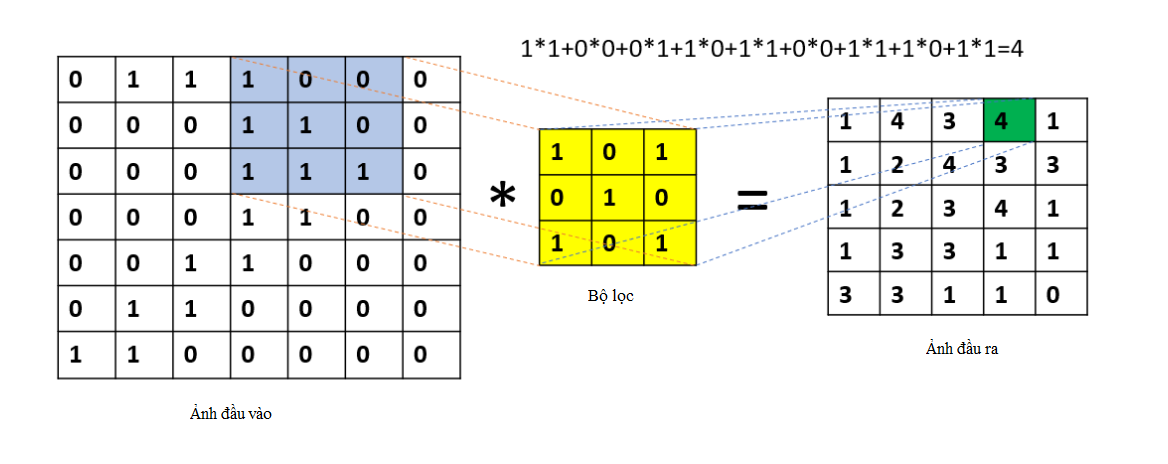
\includegraphics[width=130pt,height=110pt]{cnn.jpg}};
% %Right Arrow [id:dp363270476880974] 
% \draw  [fill={rgb, 255:red, 0; green, 255; blue, 73 }  ,fill opacity=1 ] (299,138) -- (341,138) -- (341,158) -- (369,148) -- (341,168) -- (341,158) -- (299,158) -- cycle ;

% \end{tikzpicture}
% 	\caption{Phát hiện đối tượng thông thường (Nguồn: www.cgtrader.com)}
% 	\label{fig:detect}
% \end{figure}}

% \bigskip




\end{document}